\section{Śledzenie promieni}

\subsection{Podstawowy algorytm śledzenia promieni}

Metoda śledzenia promieni pozwala określić widoczność obiektów znajdujących
się na scenie (a tym samym na generowanie obrazu) na zasadzie śledzenia umownych promieni świetlnych biegnących od obserwatora w scenę. W perspektywicznym rozumieniu sceny (a takiego dotyczy algorytm zaimplementowany na potrzeby tej pracy), pierwszym krokiem algorytmu jest wybranie środka rzutowania (nazywanego okiem obserwatora) oraz rzutni (powierzchnia, na której zostanie odwzorowana trójwymiarowa scena). Rzutnię (a właściwie interesujący nas wycinek rzutni - abstrakcyjne okno obserwatora) można podzielić na regularną siatkę, w której każde pole odpowiada jednemu pikselowi ekranu urządzenia (tzw. układ urządzenia). Kolejnym krokiem algorytmu jest wypuszczenie promienia wychodzącego z oka obserwatora, przechodzącego przez dany piksel ekranu i lecącego dalej - w scenę. Kolor piksela jest ustalany na podstawie barwy i oświetlenia najbliższego obiektu (więcej o metodach oświetlenia można przeczytać w rozdziale !TU WSTAW ROZDZIAŁ!), który został przecięty przez wysłany promień. W przypadku braku kolizji piksel przybiera barwę otoczenia. 

\begin{figure}[H]
\centering
  \caption{Rzut perspektywiczny, źródło: http://www.zsk.ict.pwr.wroc.pl}
  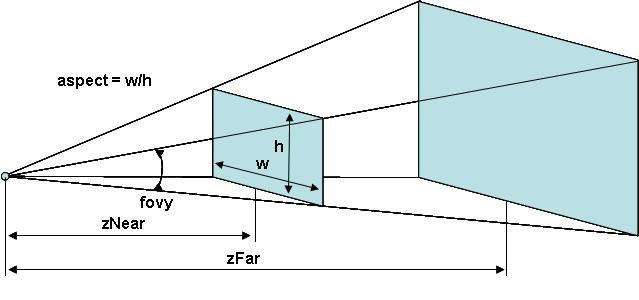
\includegraphics[width=10cm]{perspective_view.jpg}
\end{figure}

\noindent
Poniżej przedstawiono pseudokod podstawowego śledzenia promieni

\begin{algorithm}
\begin{algorithmic}
\State piksele, obiekty
\State obj = null
\State dist = max
\\
\State wybór środka rzutowania i rzutni
\\
\For{piksel in piksele}
	 \State wyznacz promień
	 \For{obiekt in obiekty}
	 \If {promień przecina obiekt i dystans $<$ dist}
    		\State obj = obiekt
    		\State dist = dystans
     \EndIf
	 \EndFor
\EndFor
\\
\State ustal kolor piksela na podstawie obj
\end{algorithmic}
\end{algorithm}

\noindent
Więcej na temat podstaw śledzenia promieni można przeczytać w \cite{foley95, suffern2007, scratch}

\subsection{Obliczanie przecięć}

Kluczowym elementem metody śledzenia promieni jest obliczanie przecięć promieni z obiektami sceny - zajmuje on znakomitą większość czasu potrzebnego na  wygenerowanie sceny \cite{suffern2007}. W związku z tym, chcąc optymalizować działanie programu, największy wysiłek wkłada się w dwa poniższe elementy:

\begin{enumerate}

\item Zmniejszenie kosztu wyznaczenia punktu przecięcia promienia z obiektem (stosowanie optymalnych czasowo algorytmów badania przecięcia)

\item Zmniejszenie liczby obiektów, dla których należy zbadać, czy dany promień je przecina (np. poprzez zastosowanie metody brył otaczających, czy wprowadzenie hierarchii sceny)

\end{enumerate}

Wyznaczenie przecięcia promienia z obiektem polega na rozwiązaniu szeregu równań zależnych od tego, z jakim obiektem szukamy przecięcia. Najczęściej scena składa się z wielu różnych wielokątów (poligonów), które w połączeniu ze sobą tworzą tzw. siatkę trójwymiarową (ang. mesh) reprezentującą dany obiekt - takie rozwiązanie daje możliwość tworzenia rozmaitych i skomplikowanych modeli 3D (podstawową składową takiego modelu nazywamy prymitywem). Najczęstszym rodzajem wykorzystywanych prymitywów (w grafice 3D) są trójkąty, gdyż da się z nich ułożyć dowolny inny wielokąt. Innym typem obiektów, z jakimi możemy szukać przecięcia, są wszelkiego rodzaju bryły, dające zapisać się raczej w postaci prostego równania, niż zbioru punktów. Popularnym, w śledzeniu promieni, przykładem takiej bryły jest kula lub torus. Poniżej przedstawiono metody badania przecięcia promieni z obiektami, które będą wykorzystywane w programie. Dokładny opis algorytmów oraz ich przykładową implementację można znaleźć w między innymi w \cite{dunn02, scratch}.

\subsubsection{Przecięcie promienia z kulą}
Dane są równania promienia i kuli mające następującą postać:
$$p = p_0 + tv$$
$$(x - x_s)^2 + (y - y_s)^2 + (z - z_s)^2 - r^2 = 0$$
gdzie
\\
$p_0$ - punkt początkowy promienia $(x_0, y_0, z_0)$ \\
$v$ - wektor kierunkowy promienia o długości 1 $(x_v, y_v, z_v)$ \\
$t$ - parametr określający odległość danego punktu, należącego do promienia, od jego początku tego promienia \\
$(x_s, y_s, z_s)$ - współrzędne środka kuli \\
$r$ - promień kuli \\
\\
Po podstawieniu równania promienia do równania kuli otrzymujemy równianie kwadratowe zależne od współczynnika t:
$$a = x_v^2 + y_v^2 + z_v^2 = 1$$
$$b = x_v(x_0 - x_s) + y_v(y_0 - y_s) + z_v(z_0 - z_s)$$
$$c = (x_0 - x_s)^2 + (y_0 - y_s)^2 + (z_0 - z_s)^2 - r^2$$
Jeżeli istnieją rozwiązania ($\Delta \geq 0$) to $t_{1,2} = -b \pm \sqrt{\Delta}$. Najczęściej interesują nas tylko rozwiązania dodatnie (dla $t < 0$ przecięcie znajduje się za promieniem). W przypadku dwóch rozwiązań dodatnich wybieramy mniejsze (bliższy punkt przecięcia). Podstawiając rozwiązanie do równania promienia otrzymamy punkt przecięcia zawierający się w powierzchni kuli.

\subsubsection{Przecięcie promienia z płaszczyzną}

Płaszczyzna nie jest prymitywem, gdyż z definicji jest ona nieskończona, jednak wyliczenie przecięcia promienia z płaszczyzną jest najczęściej pierwszym krokiem znalezienia przecięcia z dowolnym poligonem (najpierw znajduje się przecięcie z płaszczyzną wyznaczoną przez dany wielokąt, a następnie sprawdza się, czy zawiera się w nim wyliczony punkt przecięcia). Dodatkowo algorytm przecięcia promienia z płaszczyzną jest wykorzystywany w tworzeniu drzewa BSP (o którym więcej w rozdziale !TU WSTAW ROZDZIAŁ!). \\
\noindent
Dane są równania promienia i równanie płaszczyzny:
$$p = p_0 + tv$$
$$Ax + By + Cz + D = P \bullet N + D = 0$$
gdzie
\\
$p_0$ - punkt początkowy promienia $(x_0, y_0, z_0)$ \\
$v$ - wektor kierunkowy promienia o długości 1 $(x_v, y_v, z_v)$ \\
$t$ - parametr określający odległość danego punktu, należącego do promienia, od jego początku tego promienia \\
$P$ - dowolny punkt płaszczyzny \\
$N$ - wektor normalny do płaszczyzny \\
\\
Podstawiając równanie promienia (dowolny punkt promienia) za punkt płaszczyzny otrzymujemy:
$$(p_0 + tv) \bullet N + D = 0$$
$$t = -(p_0 \bullet N + D)/(v \bullet N)$$
Podstawiając $t$ do równania promienia otrzymujemy punkt przecięcia. Jeżeli $t < 0$ to płaszczyzna znajduje się za promieniem, w przeciwnym przypadku przed (gdy $t = 0$ punkt początkowy zawiera się w płaszczyźnie). Należy zwrócić uwagę, że $v \bullet N$ nie może być równe zero - jeżeli jest, znaczy to, że promień nigdy nie przecina płaszczyzny (jest do niej równoległy).

\subsubsection{Przecięcie promienia z trójkątem}

Poniżej przedstawiono dwa sposoby na znalezienie punktu przecięcia promienia z trójkątem (trójkąt jest zdefiniowany poprzez trzy znane punkty - a, b, c).


\paragraph{1. Algorytm klasyczny}\mbox{} \\

\begin{outline}[enumerate]

\1 Wyznaczenie równania płaszczyzny z trójkąta:
\2 Obliczenie wektora normalnego do trójkąta:
	$$v = (b - a) \times (c - a)$$
	$$n = v/|v|$$
\2 Wyznaczenie płaszczyzny poprzez podstawienie do równania ogólnego  dowolnego punktu będącego kątem trójkąta i wektora normalnego.

\1 Znalezienie punktu przecięcia płaszczyzny z promieniem - punkt ten nazwijmy $x$.

\1 Sprawdzenie, czy punkt przecięcia z płaszczyzną leży wewnątrz trójkąta:

\2 Punkt leży wewnątrz trójkąta, jeżeli znajduje po tej samej stronie każdej krawędzi, co punkt nie należący do tej krawędzi:
$$(b - a) \times (x - a) \bullet n > 0$$
$$(c - b) \times (x - b) \bullet n > 0$$
$$(a - c) \times (x - c) \bullet n > 0$$

\end{outline}
\paragraph{2. Algorytm Möller – Trumbore}\mbox{} \\

Algorytm ,,Möller – Trumbore'' nazwany tak na cześć swoich twórców - Tomasa Möllera and Bena Trumbore'a - jest tzw. szybkim algorytmem badania przecięcia się promienia z trójkątem bez potrzeby wyznaczania płaszczyzny, na której leży trójkąt. Algorytm ten wykorzystuje współrzędne barycentryczne. Najpierw wybieramy dowolny róg trójkąta (jeden z punktów go definiujących) - będzie on naszym początkiem barycentrycznego układu współrzędnych. Powiedzmy, że tym punktem początkowym był punkt $a$. Tworzymy dwa wektory położone na krawędziach i zaczynające się w tym punkcie $(c - a)$ i $(b - a)$ - w ten sposób, startując z punktu $a$ i przesuwając się zgodnie z wektorami (zgodnie z parametrami z zakresu od 0 do 1), możemy dostać się do dowolnego punktu należącego do trójkąta. Stąd bierze się równanie:
$$P = a + u * (c - a) + v * (b - a)$$
Należy zwrócić uwagę na dwa fakty. Po pierwsze, jeżeli któraś ze zmiennych u i v jest mniejsza od zera lub większa od jedynki, to jesteśmy poza trójkątem. Po drugie, jeżeli $u + v > 1$ to przecięliśmy krawędź BC, to również wyznaczony punkt znajduje się poza trójkątem.


Na tym etapie, znając punkt przecięcia z płaszczyzną wyznaczoną przez trójkąt, możemy w prosty sposób sprawdzić, czy dany punkt należy do trójkąta, jednak liczenie punktu przecięcia z płaszczyzną nie jest tu konieczne. Podstawiając za $P$ równianie promienia otrzymamy:

$$p + td = a + u * (c - a) + v * (b - a)$$
$$p - a = -td + u * (c - a) + v * (b - a)$$

Wartości parametrów t, v i u można w prosty sposób wyliczyć stosując iloczyn skalarny i wektorowy:

$$pvec = d \times (c - a)$$
$$qvec = (p - a) \times (b - a)$$
$$invDet = 1/((b - a) \bullet pvec)$$
$$u = ((p - a) \bullet pvec)) * invDet$$
$$v = (d \bullet qvec) * invDet$$
$$t = ((c - a) \bullet qvec) * invDet$$
Poniżej przedstawiono przykładową implementację algorytmu ,,Möller – Trumbore'' zaczerpniętą z \cite{wikiMoll}:

\begin{lstlisting}

bool RayIntersectsTriangle(Vector3D rayOrigin, 
                           Vector3D rayVector, 
                           Triangle* inTriangle,
                           Vector3D& outIntersectionPoint)
{
    const float EPSILON = 0.0000001; 
    Vector3D vertex0 = inTriangle->vertex0;
    Vector3D vertex1 = inTriangle->vertex1;  
    Vector3D vertex2 = inTriangle->vertex2;
    Vector3D edge1, edge2, h, s, q;
    float a,f,u,v;
    edge1 = vertex1 - vertex0;
    edge2 = vertex2 - vertex0;
    h = rayVector.crossProduct(edge2);
    a = edge1.dotProduct(h);
    if (a > -EPSILON && a < EPSILON)
        return false;
    f = 1/a;
    s = rayOrigin - vertex0;
    u = f * (s.dotProduct(h));
    if (u < 0.0 || u > 1.0)
        return false;
    q = s.crossProduct(edge1);
    v = f * rayVector.dotProduct(q);
    if (v < 0.0 || u + v > 1.0)
        return false;
    // At this stage we can compute t to find out
    // where the intersection point is on the line.
    float t = f * edge2.dotProduct(q);
    if (t > EPSILON) // ray intersection
    {
        outIntersectionPoint = rayOrigin + rayVector * t; 
        return true;
    }
    // This means that there is a line
    // intersection but not a ray intersection.
    else 
        return false;
}

\end{lstlisting}



\subsection{Model światła}

Główny podział modeli światła stanowią modele empiryczne i fizyczne \cite{suffern2007, falski2004}. W niniejszej pracy skupimy się na pierwszej grupie, gdyż jest ona mniej kosztowna obliczeniowo, a dająca zadowalające rezultaty - fizyczne modele światła są raczej wykorzystywane w badaniach niż w standardowych zastosowaniach grafiki komputerowej.


Najprostszym modelem światła jest oświetlenie bezkierunkowe. Wykorzystuje ono tzw. światło otoczenia (ambient light), które z definicji nie ma określonego źródła (wypełnia całą scenę) i dochodzi do każdego elementu z taką samą intensywnością.
$$I = I_{amb} * k_{amb}$$
W powyższym wzorze $I_{amb}$ oznacza intensywność światła otoczenia, a $k_{amb}$ to ,,albedo'' powierzchni przedmiotu (stosunek ilości promienia odbitego do padającego). Wartość natężenia światła liczy się najczęściej dla trzech składowych RGB, zawierających się w przedziale od 0 do 1.


Bardziej zaawansowanym modelem, bo wykorzystującym światło rozproszone (diffuse light), jest tzw. model Lamberta - dodatkowo uwzględnia on punktowe źródła światła, których promienie padają pod pewnym kątem na daną powierzchnię. Model Lamberta zakłada, że oświetlane powierzchnie są idealnie matowe, zatem światło odbite od nich rozchodzi się tak samo we wszystkich kierunkach (odbicie lambertowskie). W związku z tym nie ma możliwości otrzymania odblasków widocznych na powierzchniach błyszczących.
$$I = I_{amb} * k_{amb} + I_{dif} * d_{amb} * (N \bullet L)$$
W powyższym wzorze $N$ i $L$ są kolejno: wektorem normalnym do powierzchni, wektorem wskazującym kierunek padania światła.


Ostatnim omawianym w tym dokumencie modelem światła jest model Phonga. Wprowadza on tzw. światło kierunkowe (specular light), które uwzględnia odblaski. Model Phonga wyraża się wzorem:
$$I = I_{amb} * k_{amb} + 1/(a + bd + c^2d)(I_{dif} * d_{amb} * (N \bullet L) + k_{spec} * I_{spec} * (R \bullet V)^n)$$
gdzie $R$ i $V$ oznaczają kolejno kierunek odbicia promienia i kierunek obserwacji. Ułamek $1/(a + bd + c^2d)$ określa intensywność padającego światła w zależności od odległości od źródła ($d$ to odległość od źródła światła, pozostałe parametry są dobieranie empirycznie).

\begin{figure}[h!]
\centering
  \caption{Model Phonga, źródło: https://pl.wikipedia.org/wiki/Cieniowanie\_Phonga}
  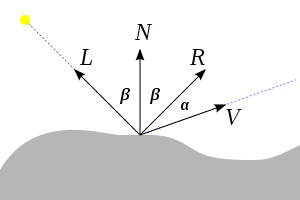
\includegraphics[width=10cm]{phong.png}
\end{figure}

\subsubsection{Cieniowanie}

Cieniowanie ma na celu stworzenie złudzenia, w którym siatka trójkątów sprawia wrażenie gładkiej powierzchni. Najpopularniejszą metodą cieniowania jest ,,Cieniowanie Gourauda'', które polega na wyliczeniu kolorów każdego wierzchołka prymitywu, a następnie interpolacji pozostałych. Takie rozwiązanie jest stosunkowo szybkie obliczeniowo, ale nie daje realistycznych rezultatów. Popularną alternatywą jest ,,Cieniowanie Phonga''. Polega ono na określeniu w każdym wierzchołku poligonu wektorów ,,normalnych'' (niekoniecznie będących normalnymi do powierzchni), a następnie wyliczeniu (poprzez interpolację) wektorów dla pozostałych punktów. Takie wektory są później wykorzystywane np. w modelu Phonga w miejsce prawdziwych wektorów normalnych. Jako że zarówno model Phonga jak i cieniowanie Phonga będą wykorzystywane w programie, którego dotyczy niniejsza praca, poniżej opisano metodę interpolacji wektorów.

\begin{figure}[h!]
\centering
  \caption{,,Cieniowanie Gourauda'' i ,,Cieniowanie Phonga'', źródło: http://www.csc.villanova.edu/~mdamian, 02.11.2017}
  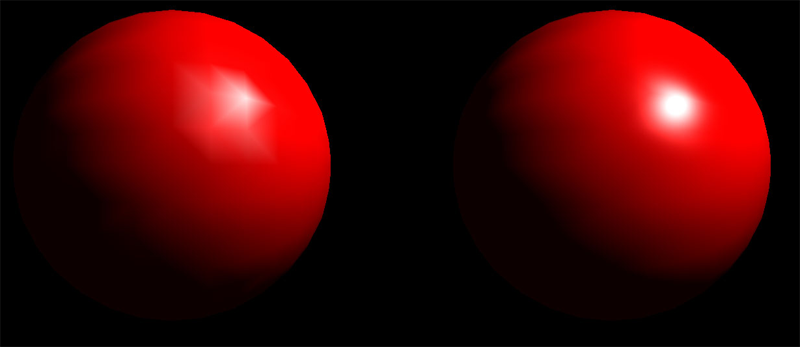
\includegraphics[width=10cm]{gouraudvsphong.png}
\end{figure}


\paragraph{Interpolacja barycentryczna}\mbox{} \\

Do interpolacji wektorów może posłużyć nam tzw. interpolacja barycentryczna. W przypadku trójkąta sytuacja prezentuje się następująco:

\begin{figure}[h!]
\centering
  \caption{Interpolacja barycentryczna, źródło: nieznane}
  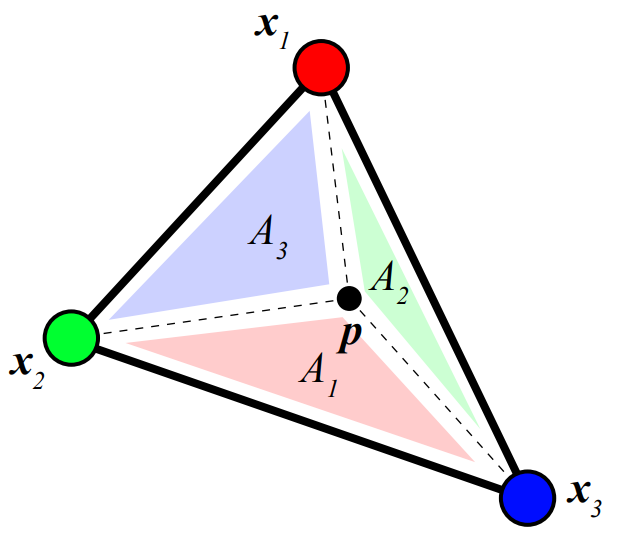
\includegraphics[width=10cm]{interpolacja.png}
\end{figure}

Na powyższym trójkącie zaznaczono punkt $p$, a następnie poprowadzono do niego proste z każdego wierzchołka. W ten sposób prymityw został podzielony na trzy mniejsze trójkąty ($A_1$, $A_2$, $A_3$), których pola zależą od odległości od kolorystycznie odpowiadających im punktów. Znając wektory normalne w tych trzech punktach i pola wszystkich trzech fragmentów możemy obliczyć, jaki wpływ ma poszczególny wektor na wektor normalny w zaznaczonym punkcje:
$$N_p = N_{x_1} * P_{A_1}/P + N_{x_2} * P_{A_2}/P + N_{x_3} * P_{A_3}/P$$
gdzie :
$N_x$ - wektor normalny w odpowiadającym punkcie.
$P$ - pole całkowite
$P_A$ - pole fragmentu

Otrzymany w ten sposób wektor należy znormalizować, ponieważ jego długość niekoniecznie wynosi jeden.

 
\subsection{Rekursywny algorytm śledzenia promieni}

Rekursywny algorytm śledzenia promieni \cite{foley95} jest rozwinięciem algorytmu podstawowego opisanego w poprzednim rozdziale. Uwzględnia on cienie, odbicia i załamania światła, dzięki śledzeniu dodatkowych promieni wysłanych z punktów przecięcia. W przypadku generowania cieni z każdego punktu przecięcia wysyła się promień w kierunku źródła światła. Jeżeli promień ten natrafi na przeszkodę, to znaczy, że punkt znajduje się w cieniu, a więc wyliczając barwę piksela (korzystając np. z modelu Phonga omówionego powyżej), korzystamy tylko ze światła otoczenia. Dla odbić, do wysłania promienia wtórnego, korzysta się z zasady, która mówi, że kąt padania równy jest kątowi odbicia. W przypadku załamania światła, określa się współczynniki jego załamania (wartości dla różnych materiałów są stablicowane i ogólnodostępne) i stosuje prawo Snelliusa \cite{snellius}:
$$sin(alpha)/sin(beta) = n_2/n_1$$
gdzie $\alpha$ - kąt padania, $\beta$ - kąt załamania, $n_1$ - współczynnik załamania pierwszego materiału, $n_2$ współczynnik załamania drugiego materiału.


W tym miejscu należy zauważyć, że nie wszystkie materiały są przezroczyste i nie wszystkie materiały odbijają światło w podobny sposób jak lustro (można w nich zobaczyć odbicia innych przedmiotów). Implementując algorytm śledzenia promieni należy wprowadzić mechanizm, który pozwala stwierdzić, jaki ułamek ostatecznego koloru piksela będzie stanowić wynik śledzenia promieni odbitych/załamanych i czy takie promienie warto wysyłać - każdy z nich znacząco wpływa na czas obliczeń, więc ich redukcja, która nie wpływa w zauważalnym stopniu na wygenerowany obraz, jest kluczowym elementem optymalizacji.


\begin{figure}[h!]
\centering
  \caption{Wizualizacja algorytmu rekursywnego, źródło: \cite{scratch}}
  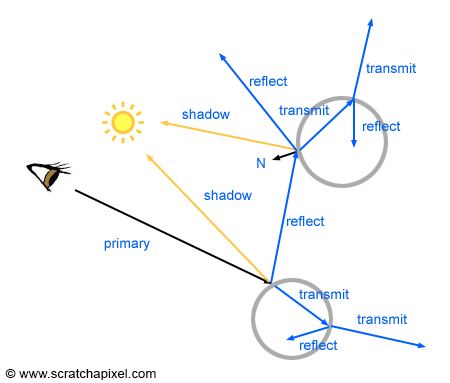
\includegraphics[width=10cm]{rekursywny.png}
\end{figure}

Rekursywny algorytm śledzenia promieni najczęściej implementuje się korzystając z funkcji rekurencyjnej \cite{suffern2007}, która przyjmuje punkt początkowy promienia, jego kierunek, oraz aktualną głębokość drzewa rekurencyjnego. Ostatni z parametrów często jest wykorzystywany w warunku stopu - po osiągnięciu określonej głębokości funkcja zwraca osiągnięty kolor.


\begin{figure}[h!]
\centering
  \caption{Wizualizacja algorytmu rekursywnego, źródło: \cite{scratch}}
  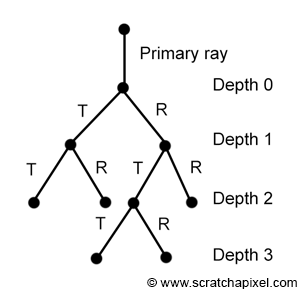
\includegraphics[width=10cm]{rekursywny_drzewo.png}
\end{figure}


\subsection{Równoległa wersja algorytmu śledzenia promieni}

Algorytm śledzenie promieni jest bardzo kosztowny obliczeniowo. Jedną ze skuteczniejszych metod przyspieszenia generowania obrazu jest jego zrównoleglenie, które w przypadku tej metody jest bardzo proste, ponieważ wygenerowanie sceny składa się z wielu obliczeń, mogących odbywać się niezależnie od siebie. Najczęściej zrównoleglenie następuje na poziomie promieni pierwotnych - zbiór pikseli (pseudokod znajdujący się w punkcie 2.1.1) dzieli się na podzbiory, które można przeanalizować równolegle. Po obliczeniu kolorów wszystkich pikseli składa się je w jeden spójny obraz. Więcej o algorytmie równoległym można przeczytać w rozdziałach !ROZDZIAŁY!.

\section{Optymalizacja algorytmu śledzenia promieni}

Tak jak to było wspomniane wcześniej, metoda śledzenia promieni jest bardzo kosztowna obliczeniowo. W związku z tym powstały metody przyspieszające, które najczęściej opierają się na redukcji testów przecięcia promieni z obiektami. Otaczając pewien model (siatkę prymitywów) bryłą, wiemy, że promień, który potencjalnie się z nim przecina, musi najpierw przeciąć daną bryłę. W ten sposób zamiast badać setki przecięć z każdym trójkątem modelu z osobna, możemy przeprowadzić tylko jeden test na bryle otaczającej. Ponadto każdą z takich brył możemy dzielić dalej na kolejne podzbiory prymitywów, a sama bryła może być fragmentem innego podziału. W ten sposób dochodzimy do czegoś, co nazywa się hierarchą obiektów.

Hierarchia obiektów ma najczęściej postać drzewa, którego korzeniem jest całą scena. Drzewo podziału przestrzeni, które zostało opisane w poprzednim akapicie, nazywamy drzewem brył ograniczających (lub otaczających), z angielskiego: bound volume hierarchy - BVH. 

\begin{figure}[h!]
\centering
  \caption{drzewo BVH, źródło: https://pl.wikipedia.org/wiki/Drzewo\_BVH}
  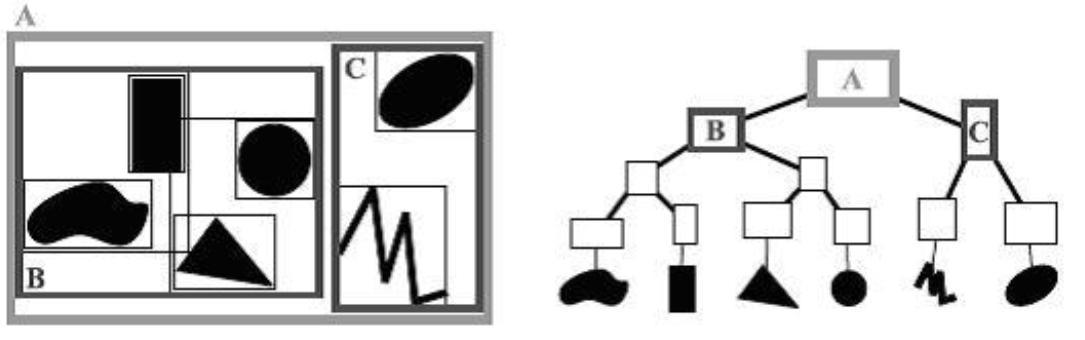
\includegraphics[width=10cm]{bvh.jpg}
\end{figure}

Podstawową zaletą drzewa BVH jest to, że w przypadku scen dynamicznych (takich, w których obiekty poruszają się) nie trzeba przebudowywać całego drzewa od początku co klatkę animacji.


Poza drzewami BVH istnieje wiele innych metod podziału podprzestrzeni. Niżej zostaną opisane jeszcze trzy z nich - wiedza na ich temat pozwoli na wybór najlepszego rozwiązania. Więcej na temat każdego z opisanych tutaj drzew można przeczytać w \cite{trees, dunn02}.

\subsection{Drzewa ósemkowe}

Budowa drzewa ósemkowego (ang. octree) polega na rekurencyjnym podziale przestrzeni na mniejsze regularne części - najczęściej sześciany.

\begin{figure}[h!]
\centering
  \caption{octree, źródło: https://en.wikipedia.org/wiki/Octreee}
  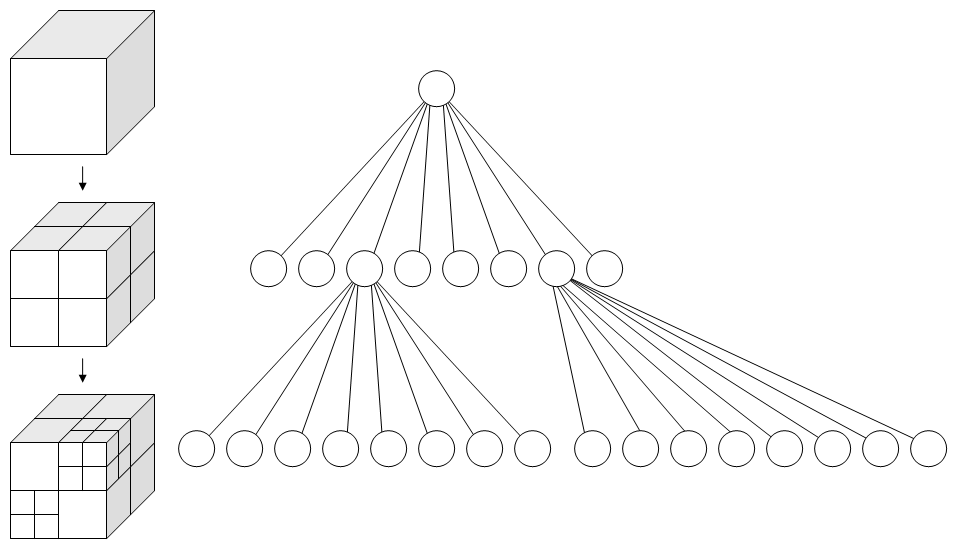
\includegraphics[width=10cm]{octree.png}
\end{figure}

Takie rozwiązanie ma znaczącą wadę w przypadku, kiedy obiekty sceny są daleko od siebie, jednak prostota drzewa ósemkowego i krótki (w porównaniu do alternatyw) czas jego budowy sprawia, że jest ono często wykorzystywane w grafice komputerowej \cite{octree1, octree2}.

\begin{figure}[h!]
\centering
  \caption{Zły przypadek dla drzewa ósemkowego}
  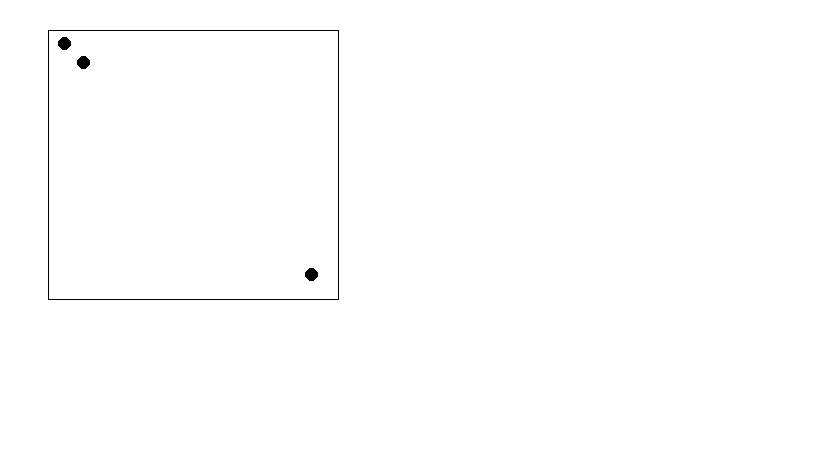
\includegraphics[width=10cm]{badoctree.png}
\end{figure}

\subsection{Drzewa K-d}

Budowa drzewa K-d (skrót od \emph{k-dimensional tree}) polega na podziale przestrzeni płaszczyznami równoległymi do osi układu współrzędnych (w przypadku trzech wymiarów są to osie x, y i z), w taki sposób aby po jednej i drugiej stronie ,,cięcia'' była podobna liczba prymitywów (jest to jedna z popularniejszych metod), a sama płaszczyzna przecinała jak najmniej figur. W ten sposób powstaje drzewo binarne.

Wybór płaszczyzny (w którym miejscu powinna ona przebiegać i do której osi powinna być równoległa) jest podstawowym elementem wpływającym na powstanie zrównoważonego drzewa. Najczęściej programiści uzależniają kierunek płaszczyzny od poziomu drzewa - w ten sposób ,,cięcie'' można wyznaczyć dzięki prostym punktom.

\begin{figure}[h!]
\centering
  \caption{Drzewo K-d dla dwóch wymiarów}
  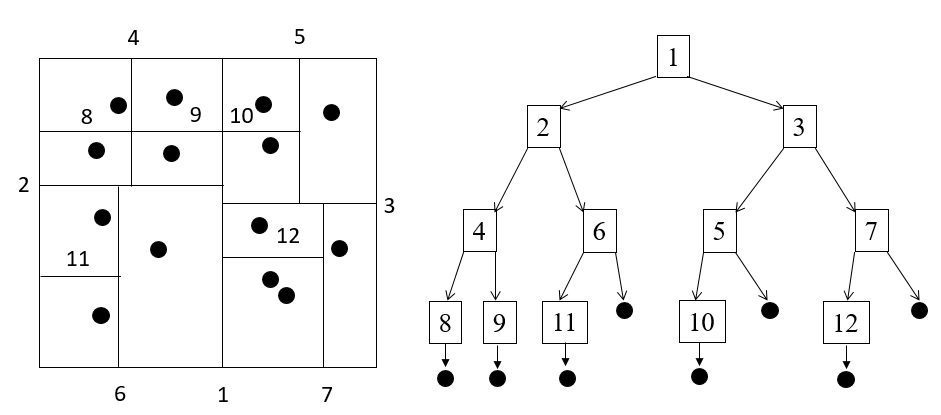
\includegraphics[width=10cm]{kd.png}
\end{figure}

Można powiedzieć, że drzewo k-d jest bardziej ogólnym przypadkiem drzewa ósemkowego, w którym przestrzeń nie musi być dzielona na takie same kształty - dzięki temu obliczenia z zastosowaniem drzewa k-d są często szybsze niż przy zastosowaniu drzewa ósemkowego. Z drugiej jednak strony czas budowania takiego drzewa jest znacznie dłuższy (szukanie optymalnego ,,przecięcia'') niż w przypadku drzew ósemkowych.


\subsection{Drzewa BSP}

Wadą drzew k-d jest możliwość cięć tylko pod trzema kątami (w przestrzeni 3D). W przypadku gdy dwa prymitywy mają wspólną krawędź będącą pod kątem do każdej z osi, nie mogą one zostać rozdzielone. Wadę tę eliminują drzewa BSP - ogólniejsza postać drzew K-d.

W każdym kolejnym kroku wybierana jest dowolna płaszczyzna (zgodnie z pewną strategią np. SAH), która dzieli przestrzeń na dwie inne podprzestrzenie. Drzewo BSP buduje się dłużej (głównie ze względu na trudność wyboru płaszczyzny podziału), ale często podział sceny jest jakościowo lepszy.


\begin{figure}[h!]
\centering
  \caption{Drzewo K-d dla dwóch wymiarów}
  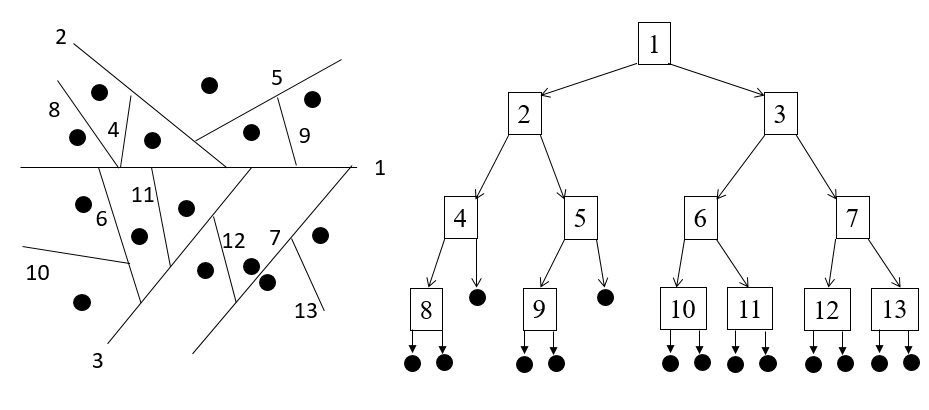
\includegraphics[width=10cm]{bsp.png}
\end{figure}


\subsection{Wybór drzewa do implementacji}

Spośród opisanych drzew, drzewa BSP i BVH intuicyjnie wydają się być najodpowiedniejszym wyborem dla metody śledzenia promieni. Na poparcie tej hipotezy warto zajrzeć do źródeł. Według \cite{bvhvsoctee} drzewo BVH jest wydajniejsze od drzewa ósemkowego (biorąc pod uwagę czas generowania sceny, a nie budowy drzewa). Jeżeli porównywać ze sobą drzewa BVH i K-d warto zajrzeć do \cite{bvhvskd1, bvhvskd2}. Autorzy wskazują na przewagę drzewa BVH, jednak uzależniają wyniki od rodzaju promieni (pierwotne, wtóre) i od definicji sceny. Wygląda na to, że jeżeli promienie często nie trafiają w żaden obiekt, to drzewo BVH jest dużo skuteczniejsze (ma to związek ze sposobem przeglądania drzew K-d). Przy scenach zamkniętych składających się z wielu trójkątów (dla mniejszych scen BVH jest najczęściej lepsze) sytuacje nie jest już taka oczywista - tendencja się odwraca. Zgodnie z przewidywaniami, potwierdzonymi przez \cite{bspvskd}, dobrze zoptymalizowane drzewo BSP jest znacznie wydajniejsze od drzewa K-d, zwłaszcza jeżeli chodzi o czas zużyty na testy badające przecięcia trójkątów z promieniami. We wspomnianym artykule zostały również przedstawione badania na temat drzewa BVH - w tym przypadku trudniej jest wykazać jednoznaczną wyższość jednego rozwiązania nad drugim. Podobnie jak było to opisane wyżej, drzewa BVH dużo lepiej działają w zamkniętych scenach (mało promieni, które nie trafiają w żaden obiekt). 

Powyższe badania potwierdza współczesna literatura fachowa i obecnie stosowane metody optymalizacji generowania grafiki. W \cite{trees} autor proponuje rozwiązania hybrydowe, w których duże otwarte przestrzenie i poruszające się obiekty zamykane są w drzewach BVH (drzewa BVH przyspieszają wykrycie kolizji, a poruszające się modele nie wymuszają przebudowy drzewa), z kolei zamknięte, spójne i statyczne elementy hierarchizuje się stosując drzewa BSP.

Na potrzeby tej pracy zostało zaimplementowane drzewo BSP - w związku z tym zostanie one dokładniej omówione niż miało to miejsce wyżej.

\paragraph{Budowa drzewa BSP}

Drzewo BSP zostało szczegółowo opisane w \cite{trees}, jednak warto również polecić adres strony\cite{bspfaq}, na której można znaleźć wiele użytecznych informacji na powyższy temat (między innymi przykładową implementację jego elementów), poniższa treść w dużej mierze bazuje na tej pozycji.

\subparagraph{Budowa drzewa}\mbox{} \\

Podstawową wersję algorytmu budowania drzewa BSP można przedstawić przy użyciu pseudokodu:

\begin{algorithm}
\begin{algorithmic}
\Function{Build}{*node, list$<$polygon$>$}
\\
\State node.plane = getBestPlane()
\State frontlist$<$polygon$>$, backlist$<$polygon$>$
\\
\For{polygon in list$<$plygons$>$}
	 \If {polygon.inFrontOf(node.plane)}
    		frontlist.add(polygon)
     \ElsIf {polygon.inBackOf(node.plane)}
     		backlist.add(polygon)
     \Else
     		...
     \EndIf
\EndFor
\\
\State Build(node.front, frontlist)
\State Build(node.back, backlist)
\\
\EndFunction
\end{algorithmic}
\end{algorithm}


Pierwszym ważnym krokiem, którego powyższy algorytm nie wyjaśnia, jest wybór płaszczyzny podziału. Najczęściej kandydatami są płaszczyzny wyznaczane przez prymitywy w wierzchołku drzewa (zgodnie z nimi, lub prostopadłe do nich i styczne do krawędzi). W najprostszym modelu wybiera się płaszczyznę, która dzieli zbiór trójkątów na jak najrówniejsze części - w ten sposób powstaje dobrze zbilansowane drzewo binarne. Popularną alternatywą takiego postępowania jest heurystyka SAH \cite{zuk2008, sah1, sah2} (ang. Surface Area Heuristic), która faworyzuje podziały na podprzestrzenie, z których jedna jest duża i zawiera niewielką liczbę prymitywów, a druga jest mała i zawiera ich dużo. Takie podejście jest uzasadnione, biorąc pod uwagę prawdopodobieństwo trafienia promienia w taką przestrzeń - może się okazać, że mniej zbilansowane drzewo będzie przeglądane krócej (mimo tego, że najgorszy przypadek jest jest dużo poważniejszy). Zastosowanie funkcji SAH zostało zaproponowane w \cite{sah1} i wydaje się najlepszym rozwiązaniem, jednak znacząco wydłuża ono czas budowy drzewa i jest trudniejsze programistycznie ze względu na potrzebę liczenia objętości w drzewie BSP; co nie jest tak proste jak w przypadku drzew K-d i wymaga dodatkowo zamknięcia całej sceny w bryle otaczającej (co pozytywnie wpływa na czas wykonania programu). Najczęściej objętości podprzestrzeni w drzewach BSP są aproksymowane prostopadłościanami.

\begin{figure}[h!]
\centering
  \caption{Płaszczyzny podziału: a - SAH, b - klasyczny podział; źródło: \cite{zuk2008}}
  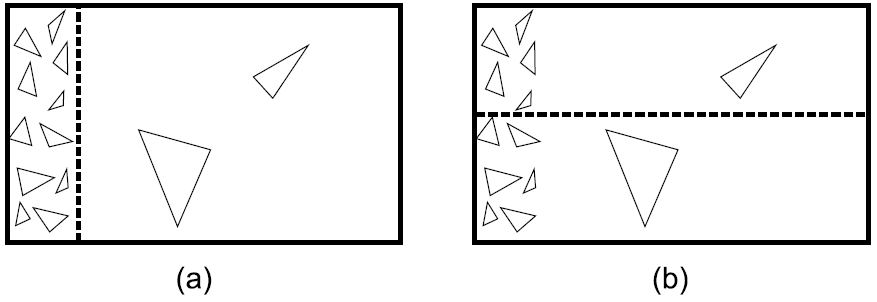
\includegraphics[width=10cm]{sah.png}
\end{figure}

Kolejnym problem pojawia się w sytuacji gdy prymityw leży na płaszczyźnie dzielącej przestrzeń lub jest przez nią przecinany. W przypadku figury leżącej na płaszczyźnie jest ona albo przypisywana do obu podprzestrzeni, albo przechowywana w danym wierzchołku. Jeżeli chodzi o poligony, które zostały przecięte to zazwyczaj dzieli się je na dwie części i przypisuje do odpowiednich potomków wierzchołka (można ich również nie dzielić i przypisać do danego wierzchołka).

Ostatnim elementem do omówienia jest warunek stopu rekurencji. Jeżeli zastosowano funkcję SAH to jest to moment, w którym dalszy podział jest nieopłacalny (metoda SAH decyduje o dalszym podziale biorąc pod uwagę przewidywany koszt przeglądania podprzestrzeni powstałych w wyniku podziału i koszt przeglądania prymitywów, jeżeli taki podział nie został dokonany). W przeciwnym przypadku najczęściej stosuje się technikę, w której wierzchołki są zamieniane w liście, jeżeli zbiór ich prymitywów jest odpowiednio mały. Można również ograniczyć drzewo co do głębokości. 

Bardzo łatwo popełnić błąd skutkujący nieskończoną rekurencją. Wybierając płaszczyzny podziału wg. prymitywów może się zdarzyć, że któryś z otrzymanych zbiorów będzie wypukły. W takiej sytuacji podział może nie być możliwy - wszystkie prymitywy mogą znaleźć się albo przed, albo za płaszczyzną dzielącą. Należy więc wprowadzić mechanizmy zabezpieczające przed taką ewentualnością.

\subparagraph{Przeglądanie drzewa}\mbox{} \\

Przeglądanie drzewa polega na rekurencyjnym sprawdzaniu, po której stronie płaszczyzny danego wierzchołka znajduje się początek promienia - od tej strony zaczniemy. Jeżeli nie znaleziono przecięcia z żadną figurą po danej stronie, a promień przecina płaszczyznę dzielącą, należy sprawdzić drugą stronę. Najgorszy przypadek to taki, w którym nie znaleziono przecięcia - algorytm trawersowania drzewa odwiedzi większość wierzchołków, co może wydłużyć czas działania programu w stopniu większym niż ma to miejsce w przeglądzie zupełnym prymitywów. Więcej informacji o przeglądzie drzewa można znaleźć w \cite{bspfaq, trees}.